\documentclass[conference]{IEEEtran}
\usepackage{cite}
\usepackage{url}
\usepackage{graphicx}
\usepackage{amsmath}

% Keep neighboring figure blocks distinct in the two-column layout.
\setlength{\floatsep}{22pt plus 3pt minus 2pt}
\setlength{\dblfloatsep}{22pt plus 3pt minus 2pt}
\setlength{\textfloatsep}{18pt plus 3pt minus 2pt}
\setlength{\dbltextfloatsep}{22pt plus 3pt minus 2pt}

\title{Post-Quantum Provenance Watermarking for Neural Network Classifiers}
% Authors sharing an affiliation can share one block.
% For another affiliation, insert \and followed by another name/address block.
\author{
  \IEEEauthorblockN{First Author Name and Second Author Name}
  \IEEEauthorblockA{\textit{Department Name, Institution Name}\\
    City, Country\\
    first@example.org, second@example.org}
}

\begin{document}
\maketitle

\begin{abstract}
A developer who receives a modified copy of a classifier may wish to establish which signed release it came from. We study this question using a convolutional classifier on CIFAR-10. The developer signs a release manifest with ML-DSA-65 and embeds a 256-bit fingerprint of that manifest in the model weights using a keyed projection and Reed--Solomon coding. An auditor with access to the weights can recover the fingerprint and check it against the signed record. Across five paired training seeds, mean test accuracy was 84.60\% for the unwatermarked baseline, 82.37\% with a binary cross-entropy watermark loss, and 84.10\% with a margin-capped hinge loss. We evaluated robustness separately on three seeds, with 252 checkpoint evaluations per design including controls. A removal required verifier rejection and an accuracy drop of at most five percentage points from the corresponding clean model. A 512-bit overwrite met this criterion for all three hinge-loss models. The binary cross-entropy design with the same code had zero successful removals in the tested configurations. The hinge objective thus recovered 1.73 percentage points of clean accuracy while introducing a measurable weakness under overwrite.
\end{abstract}

\begin{IEEEkeywords}
Model provenance, neural network watermarking, post-quantum signatures, error correction.
\end{IEEEkeywords}
\section{Introduction}
A signed release manifest lets an auditor authenticate a developer's description of a model. A harder question arises when a third party distributes a modified checkpoint: can an auditor who holds the original manifest still connect the weights to that release? Exact hashing answers whether two files are identical. A provenance watermark addresses a different question, because fine-tuning or quantization can change the checkpoint while preserving some of its learned behavior.

We investigate this question on a CIFAR-10 convolutional classifier. The developer signs a record of the release and embeds a fingerprint of that record in the weights. The signature authenticates the record, while a keyed measurement of one convolutional layer supplies evidence from the checkpoint. These steps have different failure modes: a valid signature can accompany an unrelated model, and a damaged watermark can carry statistical evidence even when decoding fails.

Our experimental question is whether reducing the classification cost of embedding preserves resistance to removal. We vary the embedding loss while holding the signed payload, carrier layer, and error-correcting code fixed. We compare accuracy across matched training seeds, then evaluate three watermark configurations under the same checkpoint modifications. The distinction between exact decoding, residual evidence, and successful removal is central to the comparison: the configuration with higher clean accuracy can also be easier to overwrite.

\section{Literature Review}
\label{sec:related-work}

\subsection{Authenticating updates and release records}
Li \emph{et al.} evaluated Dilithium, FALCON, and SPHINCS+ for authenticating model updates in federated learning. They found Dilithium the most efficient of the three in their tested settings~\cite{li2024federated}. Their verification procedure concerns a particular update exchanged during training. Campbell addressed a longer-lived object: a model bill of materials that records release information and supports post-quantum signing and attestation~\cite{campbell2026mbom}. Together, these approaches motivate a question for a downstream auditor: given a signed release record and a separately obtained, fine-tuned checkpoint, what evidence in the checkpoint links the two?

\subsection{Recovering evidence from a watermark carrier}
Uchida \emph{et al.} introduced a training regularizer that encodes a message in neural-network parameters. They recovered the watermark after fine-tuning and, in one pruning experiment, after removing 65\% of the parameters~\cite{uchida2017embedding}. This result makes the weights themselves a candidate carrier for a release identifier. It also suggests two measurements for a modified classifier: whether the watermark remains readable and whether the classifier retains useful accuracy.

Hu \emph{et al.} combined latent-space embedding, error-correcting codes, and post-quantum key encapsulation in a diffusion-model watermarking scheme. They evaluated recovery from generated images and the effect of embedding on image quality~\cite{hu2026diffusion}. Their use of redundancy motivates measuring how many bit errors a decoder can repair. The choice of carrier determines the relevant test: in our setting an auditor reads convolutional weights, and channel reordering can change a keyed projection while preserving the network's predictions~\cite{projectResults}.

\subsection{Position of this study}
Our SmallCNN implementation signs a manifest containing a CIFAR-10 dataset commitment with ML-DSA-65, a parameter set defined in FIPS~204~\cite{nist204}. It embeds a Reed--Solomon encoding of the manifest's 256-bit fingerprint in the weights. Verification checks the signature and the recovered fingerprint. This ties the checkpoint to the developer's signed claim; independent evidence would be needed to establish which data actually entered training~\cite{projectResults}.

We evaluated the choice of watermark loss while holding the payload and error-correcting code fixed. Across five paired seeds, the hinge-loss models averaged 84.10\% test accuracy and the binary cross-entropy models averaged 82.37\%. In the separate three-seed robustness evaluation, a 512-bit overwrite removed the hinge watermark on all three seeds within the five-percentage-point accuracy-drop limit~\cite{projectResults}. This tradeoff is why our evaluation reports a verification verdict alongside the predictive accuracy of each modified model.

\section{Provenance Protocol}
\subsection{Signing and embedding}
The developer commits to the ordered CIFAR-10 training set with a SHA-256 Merkle tree. Each leaf binds the sample index, label, and image bytes. A canonical JSON manifest records the root, model architecture and width, parameter count, and signing-key identifier. The developer signs the serialized manifest using ML-DSA-65~\cite{nist204}. The watermark payload is the 256-bit SHA-256 digest of those same manifest bytes. The auditor receives the signed manifest and a trusted public key separately from the model~\cite{projectResults}.

We encode the 32-byte payload using Reed--Solomon coding. RS32 appends 32 parity bytes, giving 512 binary code values; RS16 appends 16 parity bytes, giving 384. For the last convolutional layer, we average the 128 output filters and flatten the result into a vector $v$ of length $64\times3\times3=576$. A separate secret watermark key determines a reproducible matrix $X$ with entries in $\{-1,+1\}$. Each row of $X$ defines one projection score in $z=Xv$. Its sign predicts a code bit~\cite{uchida2017embedding,projectResults}.

The training objective adds $\lambda L_{\mathrm{wm}}$ to classification cross-entropy. Let $s_i\in\{-1,+1\}$ denote the target sign and $n$ the number of encoded bits. The two watermark losses are
\begin{align}
L_{\mathrm{BCE}} &= n^{-1}\sum_i \log(1+\exp(-s_i z_i)),\\
L_{\mathrm{hinge}} &= n^{-1}\sum_i \max(0,m-s_i z_i).
\end{align}
Both objectives penalize a bit whose projection has the wrong sign. Once a signed score reaches $m$, that bit contributes zero hinge loss. Binary cross-entropy (BCE) continues to reward a larger signed score. This difference motivates measuring clean accuracy and performance after an overwrite separately.

\subsection{Verification and scope}
The auditor checks the manifest signature, signed architecture and parameter count, and finiteness of the checkpoint weights. The auditor then computes the projection scores and decodes the payload, using low-confidence bytes as candidate erasures. Exact agreement with the recomputed manifest digest yields \textsc{Verified}. For an eligible code and carrier shape, the verifier can also retry extraction after channel alignment and positive scale recovery~\cite{projectResults}.

If exact recovery fails, the auditor counts raw codeword agreement in the original channel order. For RS32, agreement on at least 358 of 512 positions yields \textsc{Damaged}; the threshold corresponds to an upper-tail probability below $2^{-64}$ under independent equiprobable signs. This verdict indicates residual evidence. A failed signature check, a failed structural check, or insufficient watermark evidence yields \textsc{Rejected}. The statistical threshold applies to the specified raw comparison. We assess the behavior of the complete verification procedure separately using negative controls.

The auditor needs white-box access and the secret watermark key. Our threat model allows a third party to modify the weights. The dataset commitment lets the auditor check a supplied dataset against the signed root. Establishing that the developer actually used those data for training requires independent evidence.

\section{Experimental Design}
SmallCNN has five convolutional layers, batch normalization, rectified linear activations, max pooling, dropout, and a ten-class output layer. The width-32 configuration has 160,234 parameters. We used the standard CIFAR-10 split of 50,000 training and 10,000 test images~\cite{cifar10}. Training images were randomly cropped with four pixels of padding and randomly flipped horizontally. Test images were normalized without augmentation. The watermark training recipe used 30 epochs, batches of 128, Nesterov stochastic gradient descent with momentum 0.9, weight decay $5\times10^{-4}$, and a cosine schedule starting at 0.05. The main comparisons use $\lambda=20$ and hinge margin $m=1.5$~\cite{projectResults}.

Baseline, BCE/RS32, and hinge/RS32 accuracy comparisons use seeds 0--4. BCE/RS16 uses seeds 0--2; its accuracy cost is paired with those same baseline seeds. Robustness evaluations use seeds 0--2 for all three designs. Each design contributes 252 checkpoint evaluations including clean controls and repeated random modifications. The suite covers noise, pruning, quantization, fine-tuning, channel permutation and scaling, and watermark overwrite. A successful removal requires \textsc{Rejected} and a test accuracy drop of at most five percentage points relative to that seed's clean watermarked model. All reported counts use the saved checkpoint verdicts~\cite{projectResults}.

\section{Results}
\subsection{Accuracy and watermark strength}
Mean test accuracy was 84.60\% for the baseline, 82.37\% for BCE/RS32, and 84.10\% for hinge/RS32. Hinge improved accuracy over BCE on each of the five paired seeds (Fig.~\ref{fig:accuracy}). Across paired seeds the gain ranged from 0.92 to 2.40 percentage points, with a mean of 1.73. Relative to the unwatermarked baseline, the mean paired accuracy changes were $-2.23$ points for BCE/RS32 and $-0.50$ for hinge/RS32 (sample standard deviations 2.18 and 1.79 points, respectively). BCE/RS16 achieved 82.26\% across its three seeds, a paired cost of 2.81 points. All three designs recovered the clean payload without decoded bit errors.
\begin{figure}[!tb]
\centering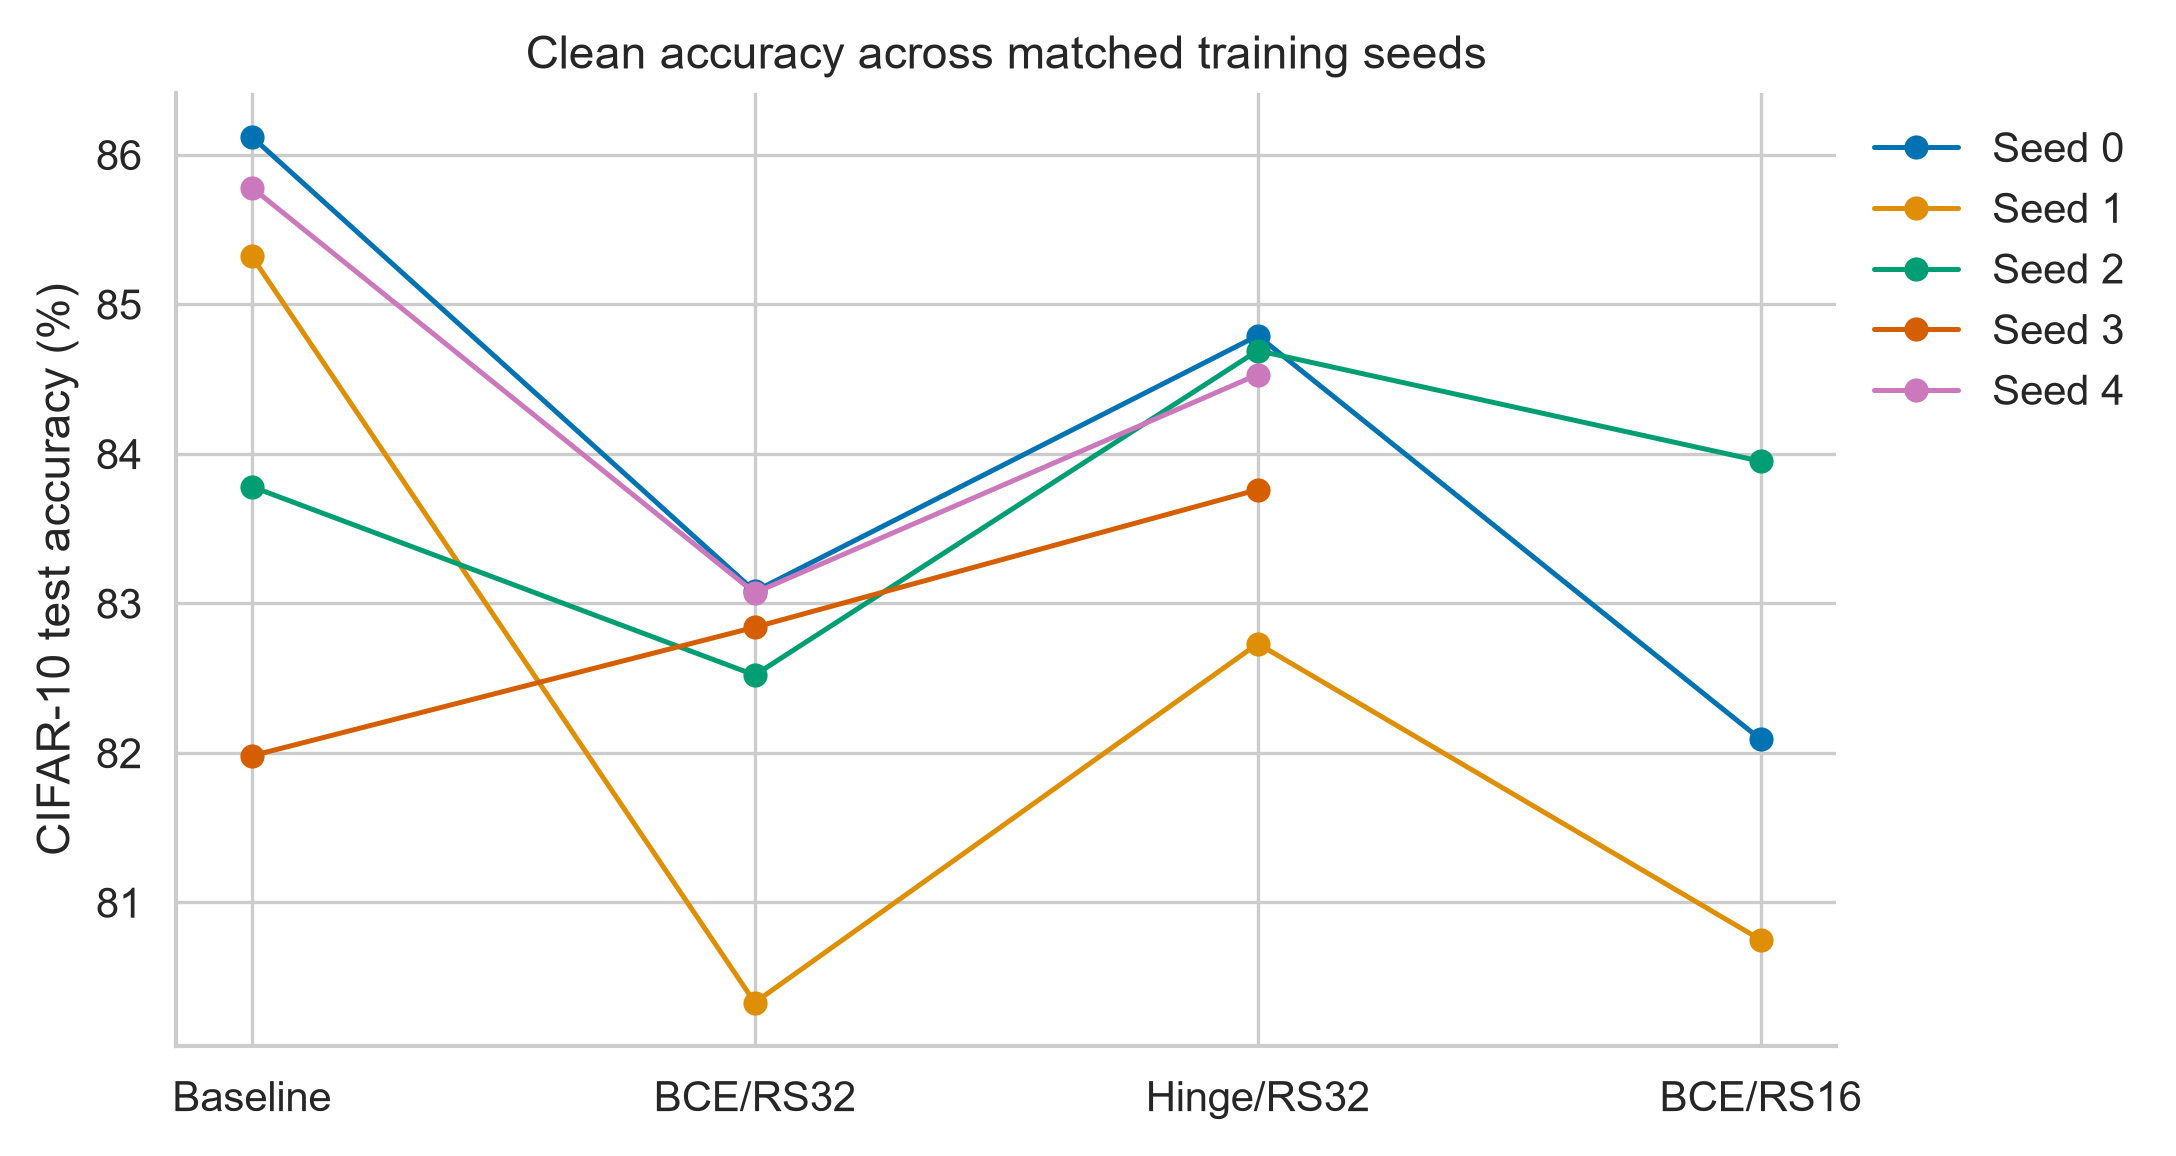
\includegraphics[width=\columnwidth]{figures/01_paired_accuracy.png}
\caption{Clean CIFAR-10 accuracy. Lines connect runs sharing a training seed. RS16 has three paired seeds.}\label{fig:accuracy}
\end{figure}

The available matched strength comparison covers seed 0. Increasing $\lambda$ from 1 to 5 to 20 raised the minimum absolute projection score from 0.02 to 1.21 to 2.25. Accuracy declined from 84.67\% to 83.19\% to 83.08\% (Fig.~\ref{fig:strength}). The margin measures how close the weakest bit lies to the decoding boundary before modification. Its increase alone does not establish resistance to overwrite.
\begin{figure}[!tb]
\centering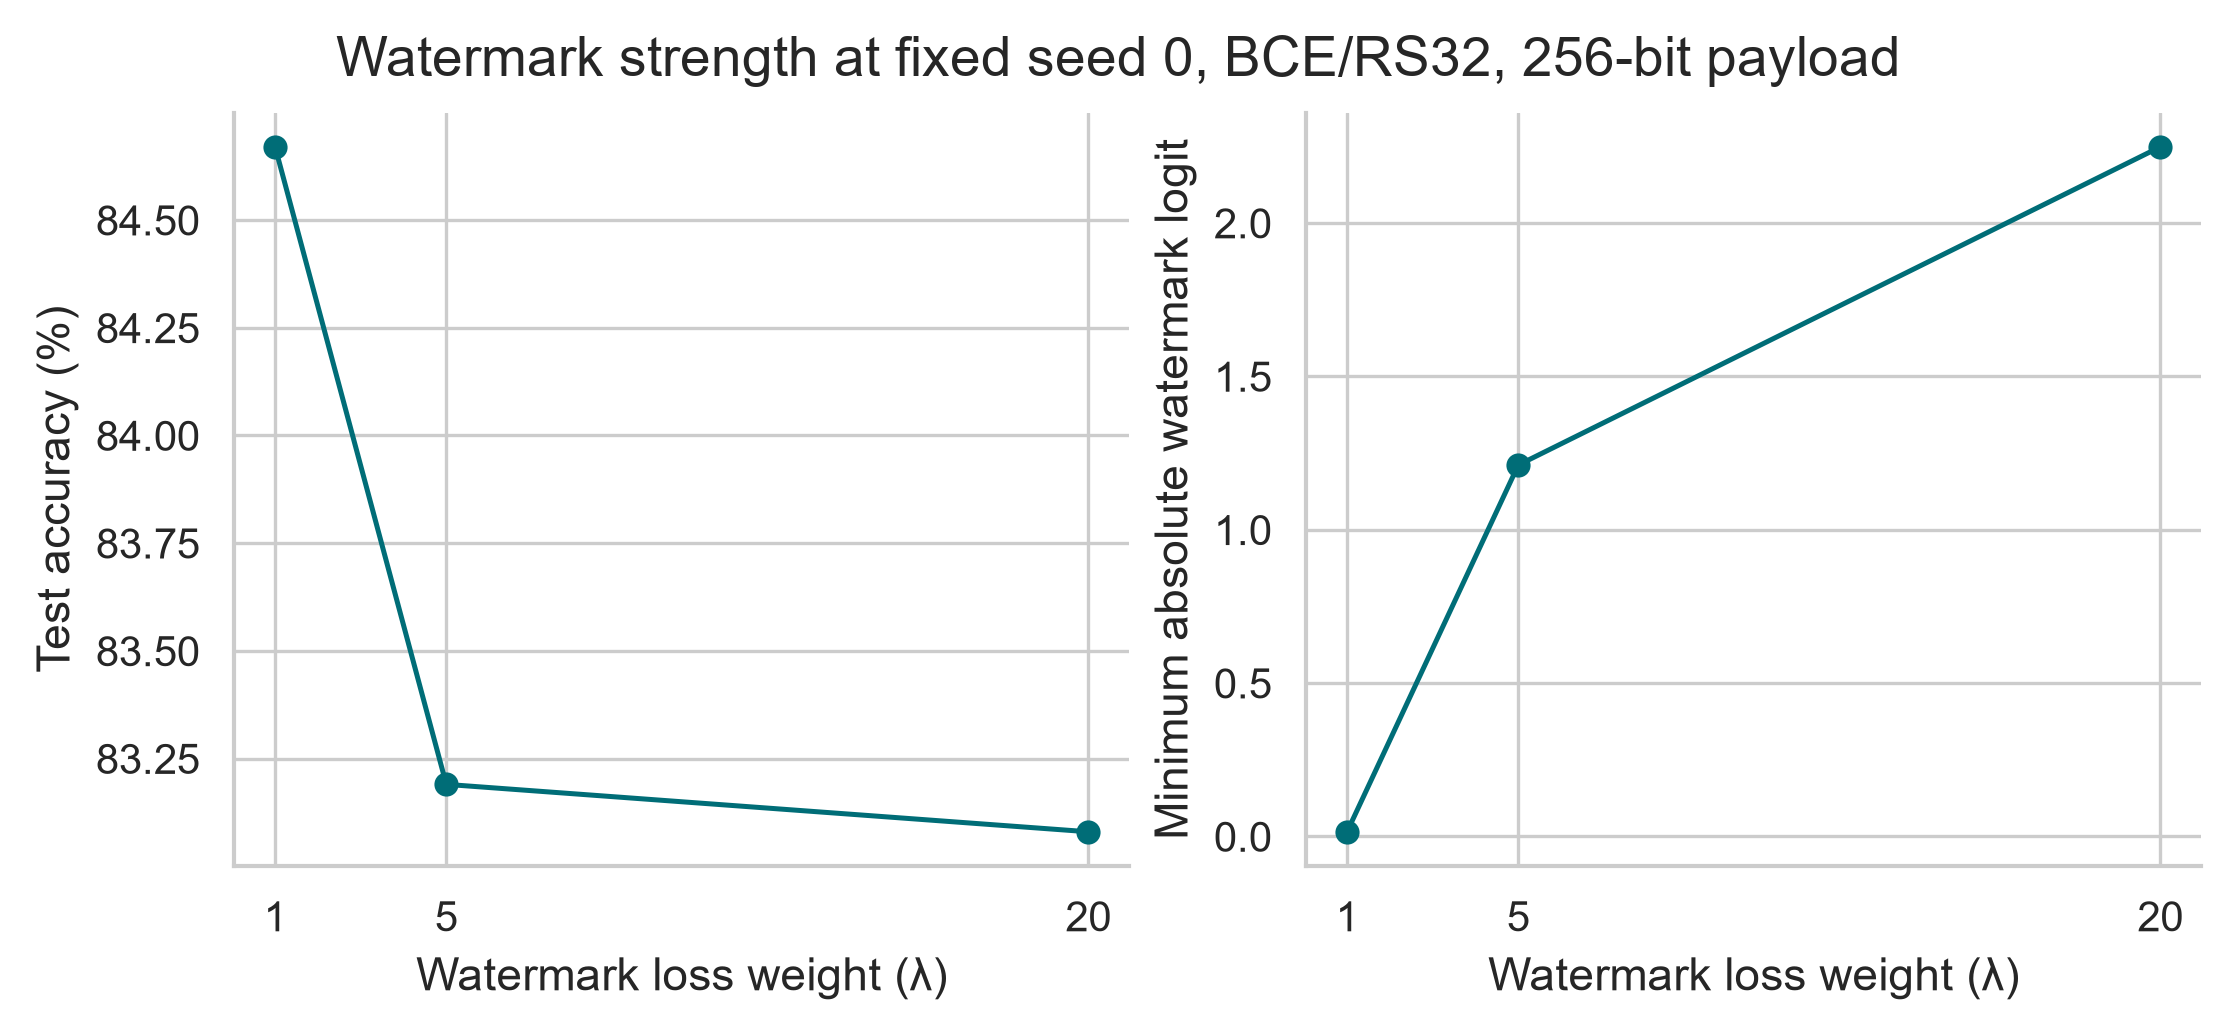
\includegraphics[width=\columnwidth]{figures/03_strength_seed0.png}
\caption{Effect of watermark strength at fixed seed, carrier layer, loss and payload. Each point represents one training run.}\label{fig:strength}
\end{figure}

\subsection{Robustness at comparable utility}
Of the 252 BCE/RS32 checkpoints, 231 verified exactly, 20 retained sufficient evidence for a damaged verdict, and one was rejected. That rejection occurred after 2-bit quantization with a large accuracy loss. BCE/RS16 yielded 240 exact and 12 damaged verdicts. Neither BCE configuration had a successful removal within the utility limit. All 108 evaluations involving channel permutation, including combined permutation and scaling, verified across the three designs.

Hinge/RS32 gave 233 exact, 13 damaged, and six rejected verdicts. Three rejections met the removal criterion. In each case a second 512-bit watermark was embedded in the carrier layer. Test accuracy fell by 4.71, 3.38, and 4.48 points for seeds 0, 1, and 2, respectively (Fig.~\ref{fig:robust}). Counting only exact recoveries would rank hinge slightly ahead of BCE/RS32 and conceal this difference. Conditioning rejection on retained model utility identifies the vulnerability.
\begin{figure*}[!t]
\centering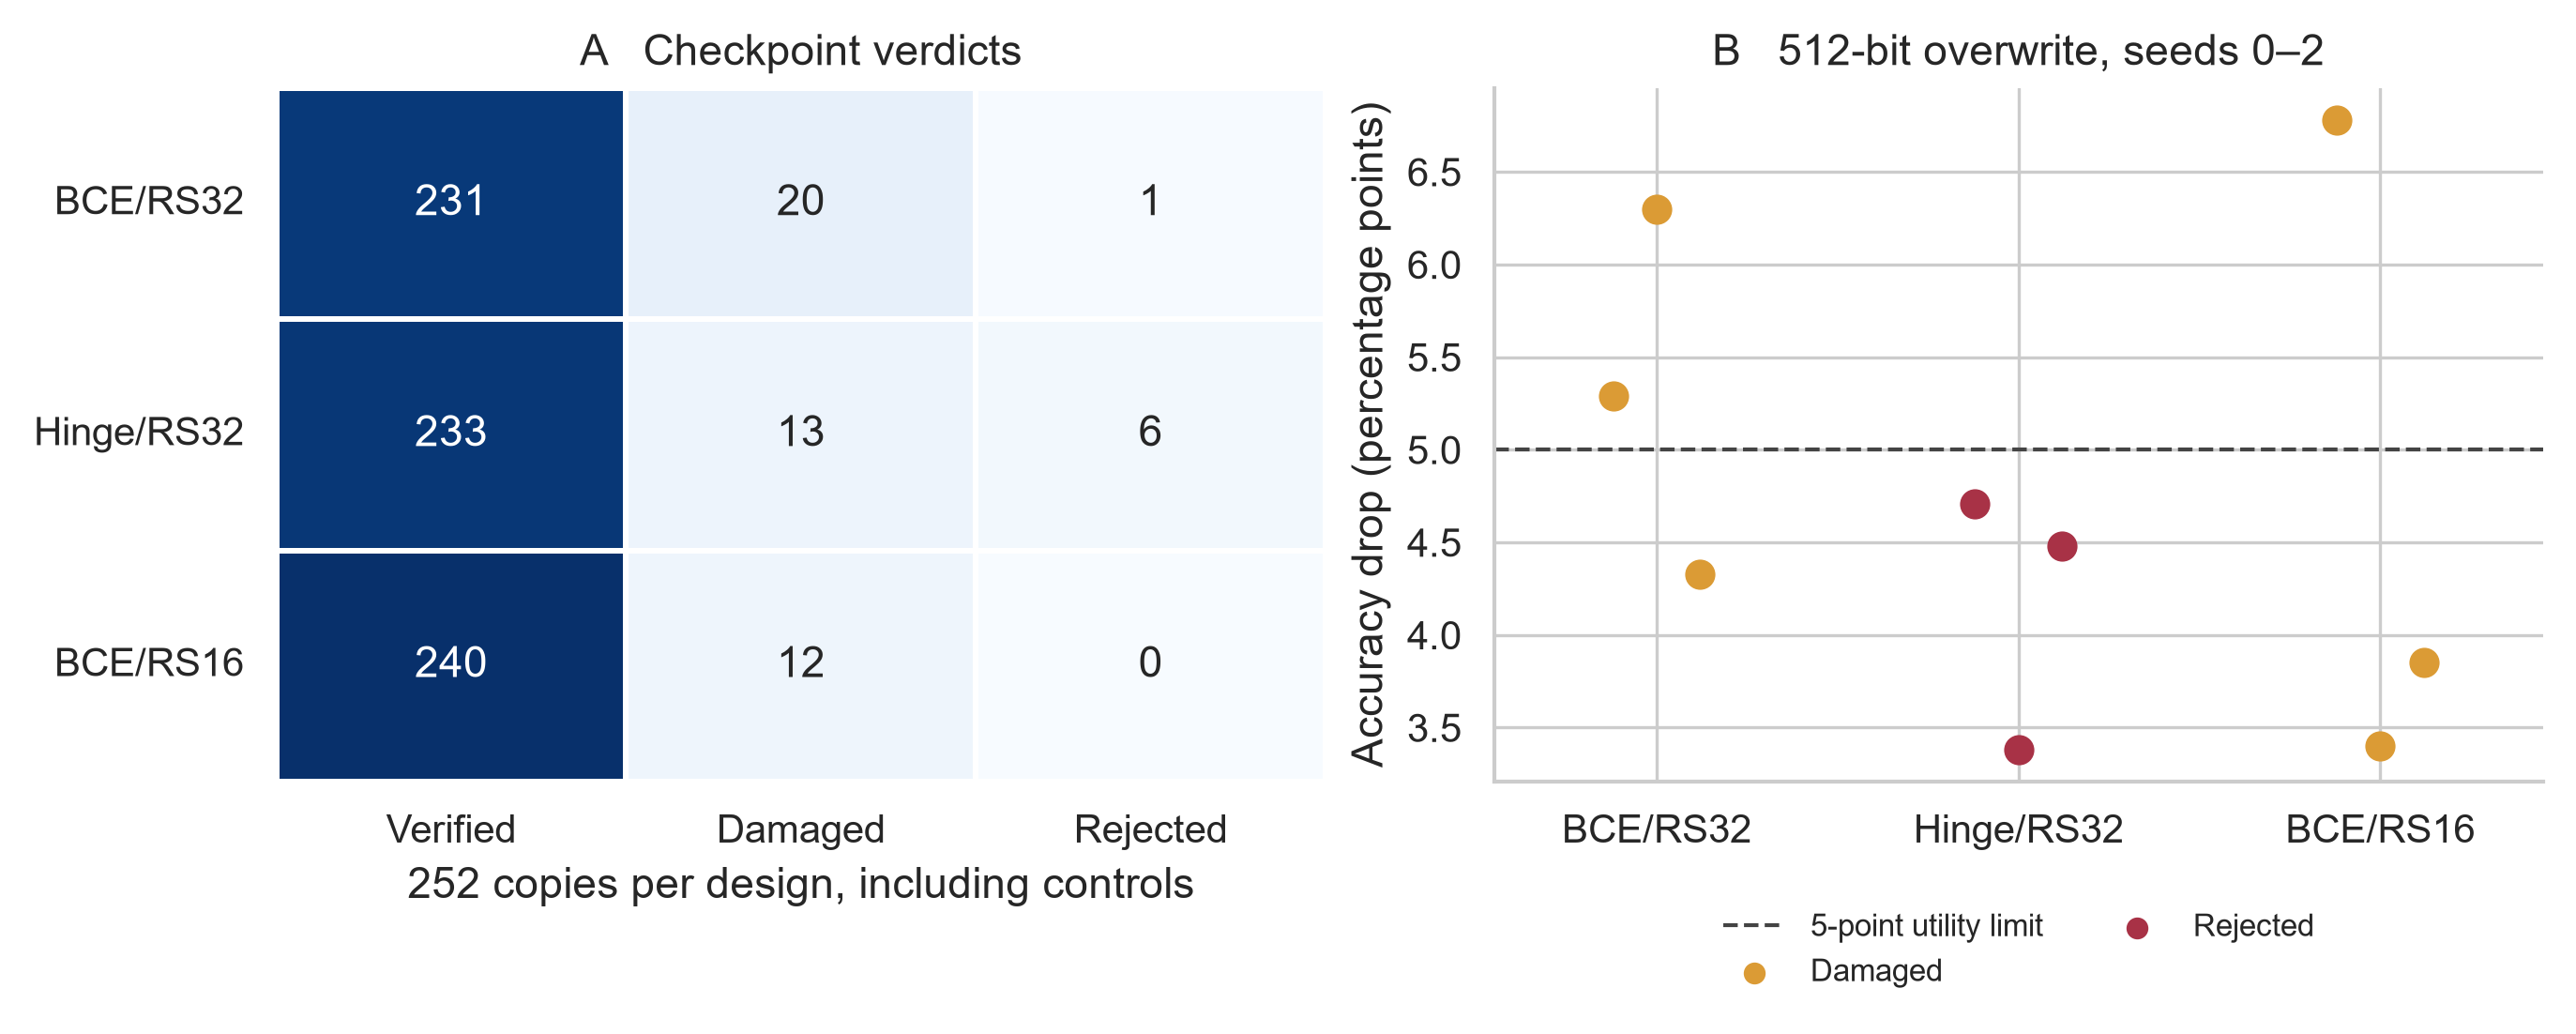
\includegraphics[width=0.91\textwidth]{figures/02_robustness.png}
\caption{Left: verifier outcomes on the same suite for each design. Right: accuracy change and verdict for each 512-bit overwrite. A rejected copy at or below the five-point limit counts as a successful removal.}\label{fig:robust}
\end{figure*}

\subsection{Error correction and negative controls}
In the original BCE/RS32 quantization evaluation, 3-bit per-tensor quantization flipped an average of 1.1\% of raw codeword positions, yet the decoder recovered the exact payload for all three seeds (Fig.~\ref{fig:ecc}). Mean classification accuracy fell by approximately 57.6 percentage points in that condition. Payload recovery and preservation of the classifier therefore require separate measurements.
\begin{figure}[!tb]
\centering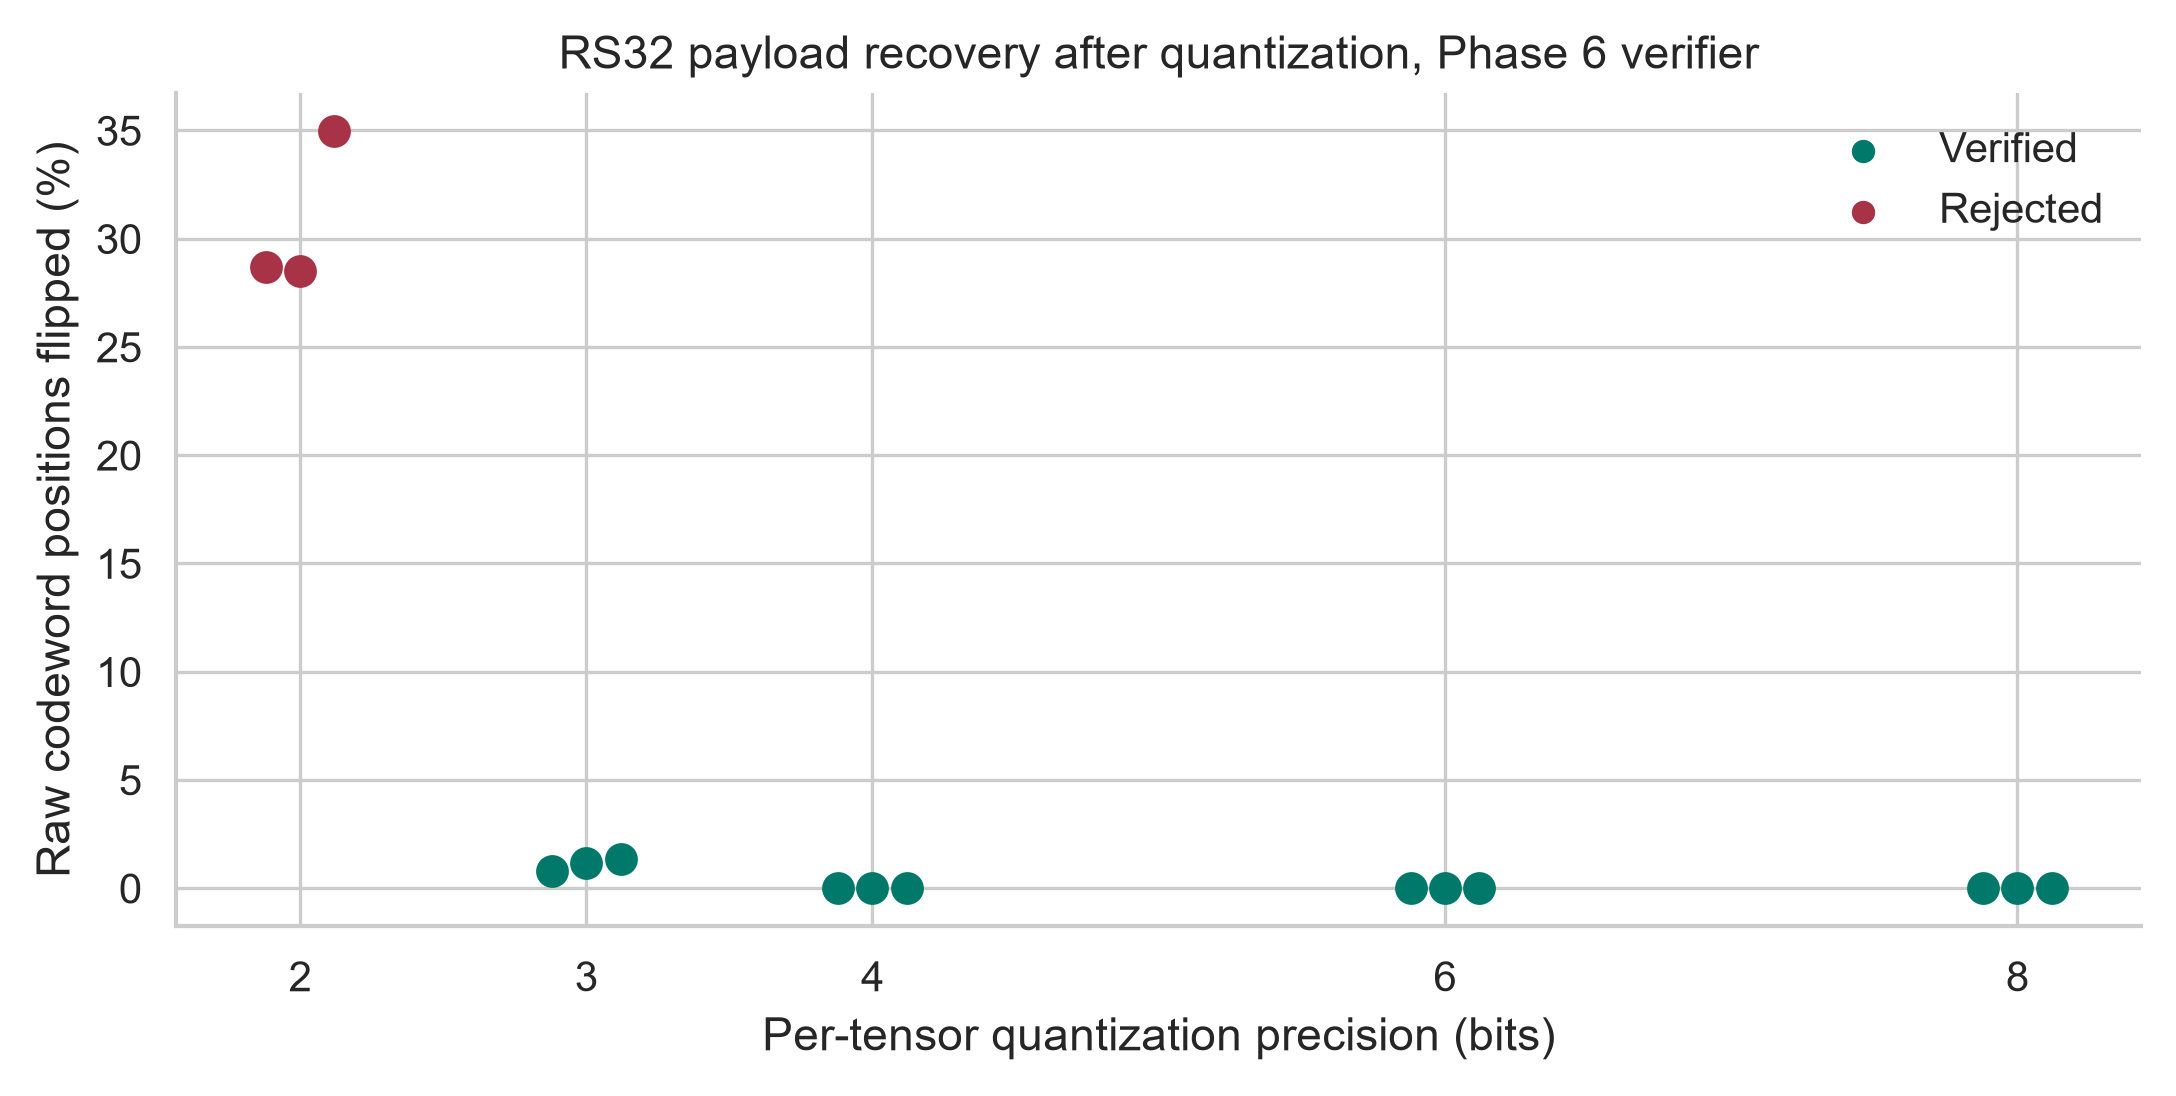
\includegraphics[width=\columnwidth]{figures/05_ecc_quantization.png}
\caption{Raw codeword errors under per-tensor quantization. Colors give the original Phase 6 verifier verdict, before the channel-alignment extension.}\label{fig:ecc}
\end{figure}

The RS32 control study comprised 724 cases, including 600 wrong-key trials and 100 random initializations. The largest raw agreement was 305 of 512 positions, below the damage threshold of 358 (Fig.~\ref{fig:null}). No case received a verified or damaged verdict. A separate set of 54 attacked baseline checkpoints also yielded zero false detections. These are empirical counts across the sampled cases; repeated trials on a shared checkpoint do not represent independently trained models.
\begin{figure}[!tb]
\centering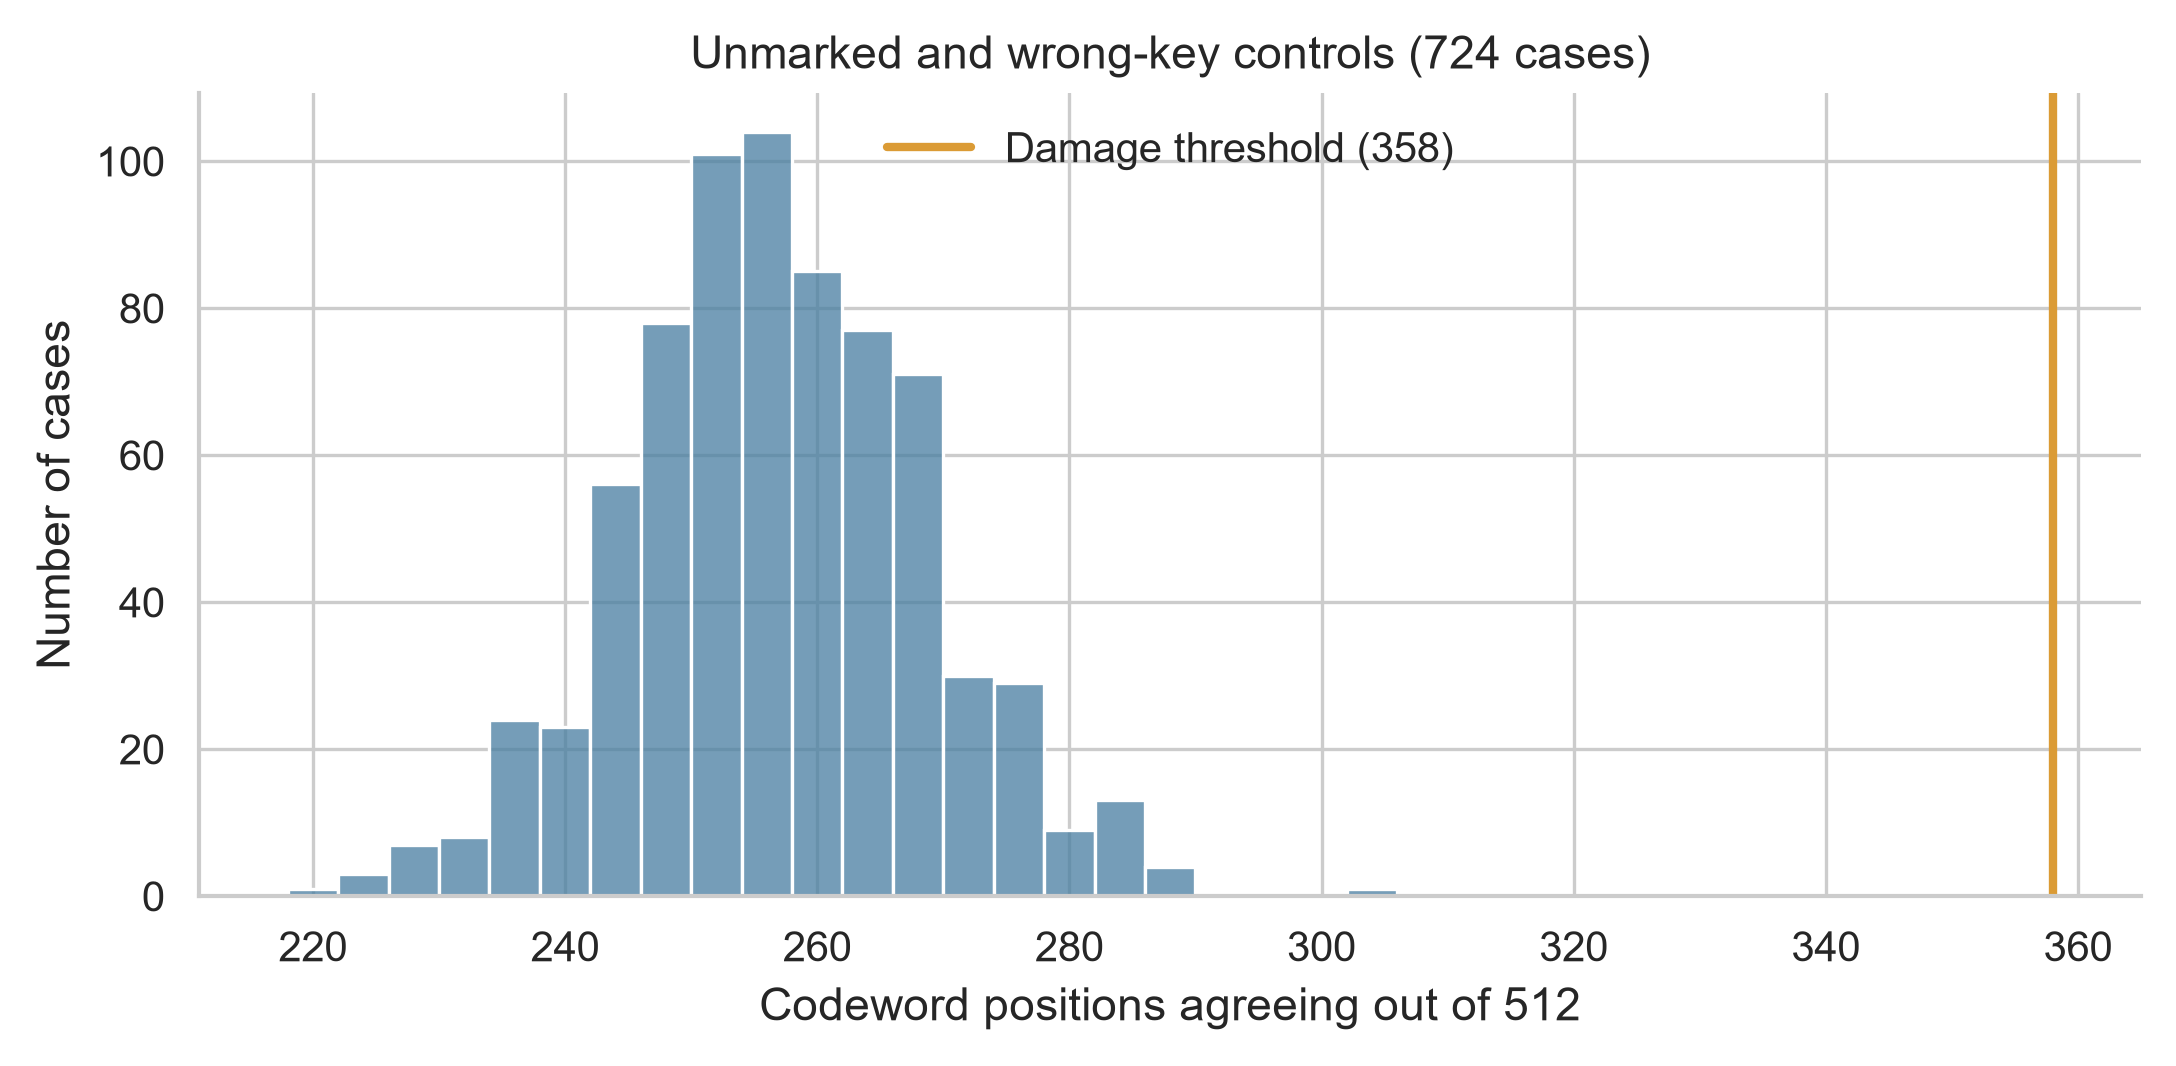
\includegraphics[width=\columnwidth]{figures/04_false_positive_controls.png}
\caption{Agreement with the signed codeword across 724 controls. The vertical line is the RS32 threshold for residual evidence.}\label{fig:null}
\end{figure}

\clearpage
\section{Discussion and Limitations}
An auxiliary comparison on two seeds assigned each code bit to the sign of a single keyed weight. This naive embedding changed clean accuracy by only $-0.09$ points on average, but six tested weight-modification configurations achieved a successful removal. The projection comparison used three seeds and more random draws per stochastic configuration. These different sample sizes limit the precision of a head-to-head rate comparison~\cite{projectResults}.

The strongest evidence for the loss comparison comes from holding architecture, code and training seed fixed. The five seed pairs establish a consistent direction for the observed accuracy change. The three overwrite trials expose a repeatable failure in this setup, but they do not yield a general removal probability. All measurements concern one classifier architecture, dataset, carrier and trusted-auditor setting. An auditor who discloses the watermark key changes the attacker's capabilities. A release intended for deployment also requires signing keys under exclusive developer control.

The current experiments do not isolate the accuracy cost of enabling error correction or varying the payload length. RS16 and RS32 both carry 256 payload bits and differ in redundancy. A matched no-code control and shorter payloads at fixed code rate remain future work. The theoretical raw-agreement threshold and the empirical controls likewise leave open a rigorous false-accept bound for the full permutation-plus-scaling search.

\section{Conclusion}
The prototype connected a signed release record to a CIFAR-10 classifier through an error-corrected weight watermark. The central result is a measured tradeoff: capping the watermark margin recovered 1.73 points of clean accuracy, while a same-layer overwrite removed the mark at useful accuracy on every tested hinge seed. Both BCE configurations resisted successful removal in the same suite, at a larger paired clean-accuracy cost. For this setting, a meaningful provenance evaluation must report the verifier's verdict and the utility of the modified classifier together.


\newpage % Start references in the adjacent IEEE column.
\begingroup
% Keep long reference entries from stretching the spaces between words.
\raggedright
\bibliographystyle{IEEEtran}
\bibliography{provenance_refs}
\endgroup
\end{document}
